\documentclass[11pt,a4paper]{article}
\usepackage[utf8]{inputenc}
\usepackage[T1]{fontenc}
\usepackage[margin=2.5cm]{geometry}
\usepackage{authblk,amsmath,amssymb,graphicx,booktabs,tabularx,array}
\usepackage[hidelinks]{hyperref}
\newcommand{\ReferenceMAGs}{5438}
\newcommand{\CBBFull}{232}
\newcommand{\HtwoCBB}{136}
\newcommand{\HtwoCBBStrict}{100}
\newcommand{\ArchaealRuBisCO}{241}
\newcommand{\DualHtwoCO}{34}
\newcommand{\HtwoCarriers}{1094}
\newcommand{\MultiHtwoMAGs}{47}
\newcommand{\JustAxioms}{38}
\newcommand{\AmbiguousSamples}{549}
\newcommand{\ForecastVisits}{409}
\newcommand{\TestVisits}{278}
\newcommand{\ConformalCoverage}{85.3\%}
\newcommand{\RankReversals}{1}

\makeatletter
\newcommand{\BacktestRows}{\@@input tables/v03_backtest.tex }
\newcommand{\ContrastRows}{\@@input tables/v04_contrasts.tex }
\newcommand{\PairedRows}{\@@input tables/v04_paired.tex }
\makeatother
\title{EQ-BioDT v0.4: evidence-aware interventions and conditional soil trace-gas scenarios for the Rub' al-Khali}
\author[1]{Robert Hoehndorf\thanks{Correspondence: robert.hoehndorf@kaust.edu.sa}}
\author[2]{Magnus Rueping}

\affil[1]{Bio-Ontology Research Group (BORG), Computer, Electrical and Mathematical Sciences and Engineering (CEMSE) Division, King Abdullah University of Science and Technology (KAUST), Thuwal, Saudi Arabia}
\affil[2]{Physical Science and Engineering (PSE) Division, King Abdullah University of Science and Technology (KAUST), Thuwal, Saudi Arabia}

\date{}
\begin{document}
\maketitle
\begin{abstract}
Linking metagenomic observations to environmental scenarios requires explicit rules for which quantities observations support and which mechanisms an intervention changes. We developed EQ-BioDT, a digital-twin prototype that combines genome-resolved pathway reasoning, conditional soil process simulations and campaign-level prediction through an executable scientific contract. Across 551 Rub' al-Khali soil metagenomes and \ReferenceMAGs{} reference genomes, the complete KEGG M00165 definition supports \CBBFull{} Calvin--Benson--Bassham (CBB) candidates, including \HtwoCBB{} with hydrogenase markers. An independently implemented module parser and OWL classification agree on every genome. Matched site--campaign comparisons associate deep sand with higher CBB carrier shares than root and surface compartments. The process model integrates water, conservative salt and trace-gas uptake within each day; a 24-member sensitivity grid reverses the ranking of single and fractionated wetting in one scenario pair. The intervention interface preserves definitions and evidence while replacing specified physical inputs, and reasoner-derived memberships admit individual reactions to a conditional resource ceiling. In \TestVisits{} future-campaign predictions, geographic and seasonal ridge regression improves on persistence, with little resolved advantage over a compartment mean; empirical nominal 90\% intervals cover \ConformalCoverage{} of observations. Published bottle experiments support an activation--diffusion moisture envelope under within-study calibration. EQ-BioDT provides a reproducible interface between annotation evidence and conditional environmental calculations, with local kinetic calibration and prospective intervention validation remaining experimental requirements.
\end{abstract}

\section{Introduction}
Desert microorganisms use atmospheric trace gases as energy sources, and some couple this metabolism to carbon fixation \cite{ji2017atmospheric,leung2020energetic,jordaan2020gobi}. Metagenomic observations identify genes and their distribution among reconstructed genomes. Soil trace-gas exchange additionally depends on water availability, pore transport, enzyme activity and substrate supply. A model that uses these observations must distinguish evidence for a genomic pathway from measurements of its realized flux.

Existing tools such as DRAM and METABOLIC infer metabolic potential from genome annotations and summarize contributions to biogeochemical processes \cite{shaffer2020dram,zhou2022metabolic}. Process models describe moisture-dependent biological and transport limitations on hydrogen uptake \cite{bertagni2021moisture}. Combining these representations raises a separate problem: a biological inference must retain its evidence and measurement meaning as it enters a physical calculation. A genome-level pathway conjunction, for example, requires its components in the same genome. Adding community-level marker abundances cannot establish this conjunction. Likewise, admitting a carbon-fixation reaction does not admit every possible energy source for that genome.

Ontologies make such definitions and their consequences explicit. OWL class expressions represent pathway alternatives, conjunctions and overlapping carrier sets, and a reasoner can provide source-axiom justifications for membership \cite{owl2direct2012}. These definitions remain fixed when a physical scenario changes. Structural causal models instead specify mechanisms whose inputs or assignments change under a prescribed intervention \cite{pearl2009causality}. Distinguishing these roles is particularly useful for broad treatments such as wetting or compaction, whose effects depend on the version of treatment, including pulse timing or post-disturbance pore properties \cite{vanderweele2013multiple}.

We implemented this separation in EQ-BioDT v0.4.0, a digital-twin prototype for soil trace-gas processes in the Rub' al-Khali. The software binds genome classifications to annotation evidence, evaluates specified forcing regimes through a shared water and salt state, and maintains a separate prediction task for marker genome equivalents. We evaluate annotation-rule agreement against an independent implementation, matched compartment contrasts, numerical convergence, future-campaign prediction and a published moisture-response dataset. The contribution is an auditable interface between these components: the same evidence and equations give the same numerical answers in a flat implementation, while the ontology supplies explicit membership semantics and explanations.

\section{Results}
\subsection{Genome-resolved module support and compartment associations}
The complete M00165 annotation rule supports \CBBFull{} of \ReferenceMAGs{} reference MAGs. Its sedoheptulose regeneration requirement includes either the sedoheptulose-bisphosphatase route or the transaldolase route. Among the supported genomes, 149 have the transaldolase alternative without an annotated sedoheptulose bisphosphatase. These are distinct biochemical routes; a transaldolase variant of the Calvin cycle has experimental precedent \cite{frolov2019transaldolase}. An independent parser evaluated the pinned KEGG module expression directly against the original KO table and agreed with both the production annotation screen and OWL classification for all \ReferenceMAGs{} MAGs.

The full module rule and hydrogenase-marker conjunction yield \HtwoCBB{} candidate genomes, of which \HtwoCBBStrict{} meet the declared completeness and contamination screen and \DualHtwoCO{} also carry a form-I CO-dehydrogenase marker. A single Rubisco-marker screen includes 1,078 MAGs, while Rubisco plus phosphoribulokinase includes 416. The additional genomes have incomplete support under the full module rule; these comparisons measure annotation-rule differences. Of \ArchaealRuBisCO{} archaeal Rubisco-positive MAGs, two also have phosphoribulokinase annotations. Domain assignment and a Rubisco KO alone leave Rubisco form and physiological function unresolved.

Genome linkage also determines how carrier abundances combine. The \HtwoCarriers{} hydrogenase-carrier MAGs include \MultiHtwoMAGs{} with multiple screened hydrogenase groups, so summing group-specific carrier shares counts those genomes more than once. Without genome linkage, hydrogenase and CBB marginal shares leave a nonzero interval of possible overlap in \AmbiguousSamples{} of 550 samples with usable mapping data. The genome-resolved intersection supplies an exact share relative to this reference catalogue and mapping measure. One of the 551 samples lacks a usable mapped composition and remains unavailable.

Deep sand has the highest median mapped CBB carrier share: 8.61\%, compared with 6.00\% in surface sand and 5.30\% in root samples. To separate this association from unequal sampling across sites and campaigns, we averaged replicates within site--campaign--compartment groups and compared paired compartments. Deep sand exceeded roots by 4.38 percentage points across 107 matched site--campaign groups, with a site-bootstrap 95\% interval of 2.91--6.00 points. The hydrogenase-plus-CBB intersection showed the same ordering in paired comparisons (Table~\ref{tab:contrasts}). These contrasts characterize relative mapping weights in the sampled cohort.

\begin{table}[ht]
\centering\small
\caption{Matched compartment differences in percentage points of mapped reads. Replicates are averaged within site and campaign. Intervals resample sites, retaining their paired visits (2,000 draws). Root denotes the plant-root compartment.}
\label{tab:contrasts}
\begin{tabular}{llrrr}\toprule
Endpoint & Contrast & Pairs & Mean difference & 95\% interval\\\midrule
\ContrastRows
\bottomrule\end{tabular}
\end{table}

\subsection{Evidence-gated reactions and specified physical interventions}
OWL classification yields membership sets whose identities are bound to the source evidence, ontology and rule version. The public resource-ceiling query reads these exported entailments. Hydrogenase-plus-CBB membership admits a conditional carbohydrate-synthesis calculation; CO oxidation additionally requires CO-carrier membership. A regression case with hydrogenase-plus-CBB support but no CO marker therefore assigns zero CO-respiration flux even when CO supply is positive. This is an evidence-admission rule: an unentailed reaction is excluded from the calculation without asserting biological absence.

The reasoner reports a consistent ontology with no unsatisfiable named classes and verifies a subset-minimal \JustAxioms{}-axiom explanation for an example hydrogenase-plus-CBB candidate. A deliberately conflated observation endpoint produces a verified three-axiom contradiction. These checks establish consequences of the supplied axioms. The independent KEGG evaluation establishes agreement with the pinned annotation rule; neither check supplies experimental activity labels.

For physical scenarios, the intervention interface pairs a baseline trajectory with specified changes to daily water, NaCl, evaporation or temperature inputs, or prescribed post-disturbance porosity and retention parameters. Both regimes share the initial state, genomic evidence and constitutive definitions. Derived uptake, carbon removal and annotation membership are excluded as clamp targets. Each result identifies the replaced inputs and fixed evidence and model versions. A same-input comparison with direct simulation gives identical trajectories, while invalid targets and pore-incompatible initial states are rejected.

\subsection{Resolving within-day uptake changes wetting comparisons}
The process layer combines water-potential activation and gas diffusion in a homogeneous soil layer. Uptake falls to zero below the dry activation threshold and at pore saturation, with an interior moisture optimum controlled by the retention relation (Fig.~\ref{fig:process}A). Water and conservative NaCl inventories persist between days. Gas calculations become unavailable when saline conditions leave the dilute model domain, while mass-balance accounting continues.

We integrated gas uptake at subdaily midpoints to represent the interval between wetting and evaporative drying. With 12~mm total water, a 14-day duration and 1~mm~day$^{-1}$ evaporation, daily additions produce 2.87~$\mu$mol~H$_2$~m$^{-2}$ at the reference parameters. The integrated uptake is positive even when daily endpoints fall below the activation threshold. Refining the default 96 steps per day to 384 changes reference-scenario uptake by at most 0.027\% across the intact, single-pulse, four-pulse and daily-pulse schedules.

Wetting preferences depend on the assumed process parameters. Across 24 combinations of retention exponent, dry threshold, activation shape and kinetic multiplier, the uptake ordering of one 12~mm pulse and four 3~mm pulses reverses. Both exceed the daily-pulse schedule throughout this grid. The intact control belongs to every four-objective Pareto set because it requires no added water or disturbance; the preferred wetting schedule varies among members (Fig.~\ref{fig:forecast}B). The sensitivity grid therefore supports conditional comparisons of treatment versions.

To evaluate the moisture-response shape against observations, we fitted exponential rates to 746 concentration measurements from 77 bottle incubations reported by Reji and colleagues \cite{reji2025h2sink}. A nonnegative amplitude times an activation--diffusion envelope reduced mean held-replicate RMSE by 54--80\% relative to a diffusion envelope in the three soils (Fig.~\ref{fig:process}B). The activation threshold was informed by the same study. This comparison evaluates a within-study moisture envelope, with amplitude refitted for each soil and training split.

\begin{figure}[ht]
\centering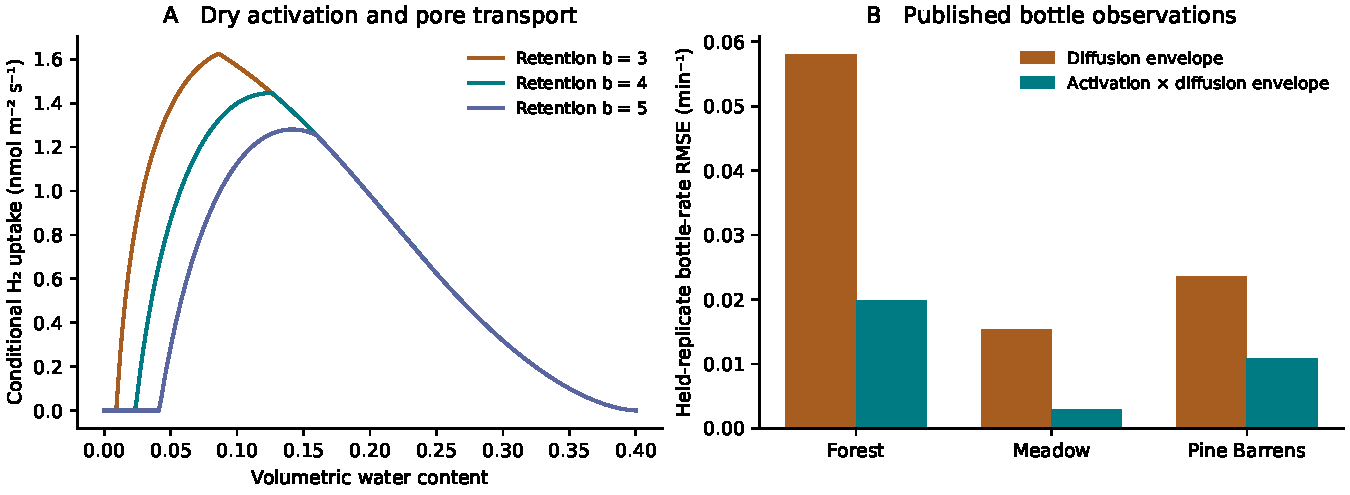
\includegraphics[width=\textwidth]{figures/process_validation.pdf}
\caption{Moisture response and published bottle observations. (A) Conditional reaction--diffusion uptake for a 0.1~m layer, porosity 0.4 and reference hydrogen reaction coefficient 0.001~s$^{-1}$ across three retention exponents. (B) Mean of held-replicate bottle-rate RMSEs for a diffusion envelope and an activation--diffusion envelope. The fixed activation threshold is informed by the same published study; the bottle comparison evaluates the envelope rather than the full soil simulator.}
\label{fig:process}
\end{figure}

\subsection{Future-campaign capacity prediction}
The prediction task comprises \ForecastVisits{} dated site--compartment--campaign means, including \TestVisits{} held-out visits in campaigns 2--5. Ridge regression using location, season and compartment has lower error than persistence in each test campaign, while the compartment mean has lower error in campaigns 2 and 4 (Table~\ref{tab:forecast}). Across all held-out visits, the paired RMSE difference between ridge and persistence is $-0.055$ on the $\log(1+\mathrm{GE})$ scale, with a site-bootstrap interval of $[-0.091,-0.019]$. The corresponding difference from the compartment mean is $-0.006$, with an interval spanning zero (Table~\ref{tab:paired}). Compartment therefore explains much of the predictable structure in this benchmark.

\begin{table}[ht]
\centering\small
\caption{Future-campaign RMSE on $\log(1+\mathrm{GE})$ and ridge coverage of nominal 90\% empirical residual intervals. Training observations precede the first collection date in each test campaign.}
\label{tab:forecast}
\begin{tabular}{rrrrrrr}\toprule
Campaign & Visits & Geog./season & Persistence & Comp.\ mean & Global mean & Coverage\\\midrule
\BacktestRows
\bottomrule\end{tabular}
\end{table}

\begin{table}[ht]
\centering\small
\caption{Paired overall RMSE differences between ridge and each baseline across \TestVisits{} visits at 58 sites. Negative differences favour ridge. Percentile intervals use 2,000 site-bootstrap draws.}
\label{tab:paired}
\begin{tabular}{lrr}\toprule
Baseline & Ridge minus baseline & 95\% interval\\\midrule
\PairedRows
\bottomrule\end{tabular}
\end{table}

Nominal 90\% intervals from site-held-out training residuals cover \ConformalCoverage{} of future-campaign observations. Coverage differs across compartments: 81.0\% in deep sand, 88.7\% in roots and 82.5\% in surface sand. These empirical intervals under-cover in the temporal test. The software retains frozen forecast inputs and checksums, allowing subsequently collected observations to be scored against predictions issued before their collection \cite{dietze2018forecasting}.

\begin{figure}[ht]
\centering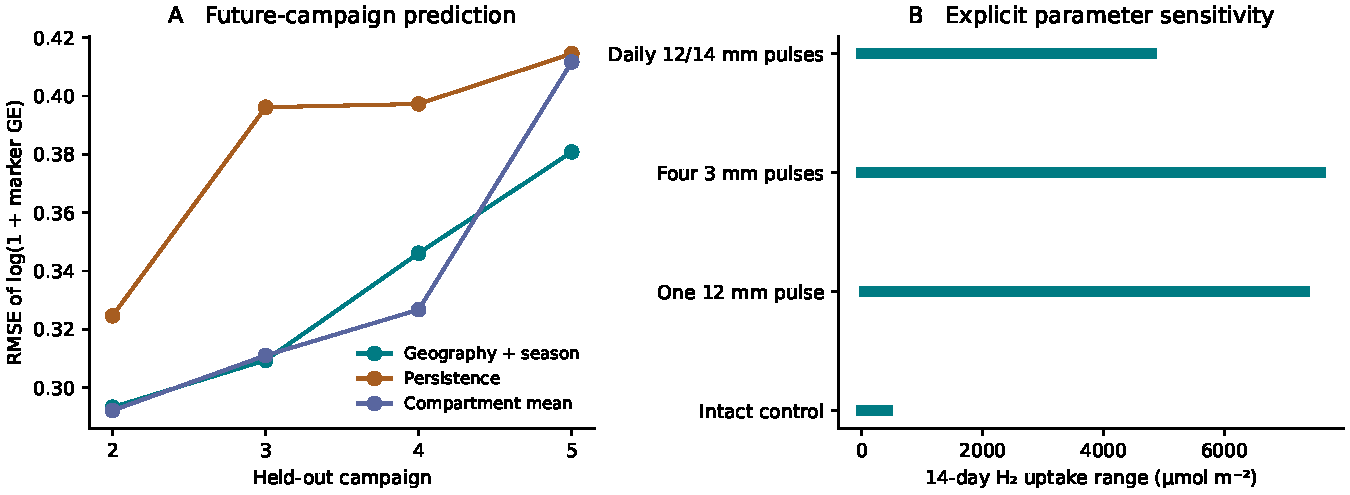
\includegraphics[width=\textwidth]{figures/forecast_scenarios.pdf}
\caption{Prediction and scenario sensitivity address different endpoints. (A) Future-campaign RMSE for marker genome equivalents. (B) Range of conditional 14-day hydrogen uptake over 24 parameter combinations for four water schedules. Parameter members represent sensitivity assumptions rather than posterior probabilities.}
\label{fig:forecast}
\end{figure}

\section{Methods}
\subsection{Evidence inputs and module semantics}
The analysis starts from 551 metagenomes, \ReferenceMAGs{} reference MAGs, corrected post-refinement KO annotations, MAG quality and GTDB taxonomy, trace-gas marker assignments, CoverM mapping percentages, read-screen genome equivalents and curated collection dates. The versioned input snapshot includes each of these analysis inputs and checksums. Sequencing, assembly and primary annotation precede this analysis boundary. Genome equivalents use the screened marker-gene read counts and single-copy-gene normalizer, with a 60\% identity floor. They denote relative gene-copy capacity.

For mapped-read weight $w_{ig}$ of MAG $g$ in sample $i$, the share of a carrier set $A$ within reference set $G$ is
\begin{equation}
q_i(A)=\frac{\sum_{g\in A}w_{ig}}{\sum_{g\in G}w_{ig}}.
\end{equation}
This share is unavailable when the denominator is zero or any required mapping weight is nonfinite. The evidence builder checks unique sample--MAG pairs, nonnegative weights, reference membership and closure of mapped plus unmapped percentages to $100\pm0.02\%$. Mapped-MAG Shannon entropy uses the same normalized weights. Genome equivalents, read shares, DNA recovery, membrane integrity, biomass and activity are separate endpoints \cite{carini2016relicdna,lennon2018relicdna}.

The pathway rule implements the 11 conjunctive requirements of KEGG M00165 as retrieved on 28 October 2026. Alternatives within a requirement are disjunctive; K01602 is optional in the module definition. The regeneration branch accepts K01100, K11532 or K01086 for the bisphosphatase route, or K00616 or K13810 for the transaldolase route. The grouping expresses alternative support for the module requirement; the two routes retain their distinct biochemical meanings. A separate parser evaluates the original KEGG expression, including parentheses, alternative branches, complexes and optional components, against the full source KO table without importing the production step dictionary.

We encode each MAG as an OWL class with existential restrictions for its observed KOs and marker guilds. The CBB-support class is the intersection of the requirement classes. Hydrogenase and CO carrier classes derive from the respective marker hierarchies; their intersections with CBB support define candidate eligibility. The declared quality subset requires completeness at least 90\% and contamination below 5\%, without claiming the complete MIMAG high-quality criteria. Domain assertions and a coarse four-bucket phylum partition support the exported ontology; detailed GTDB taxonomic summaries are tabular annotations rather than a complete imported taxonomic hierarchy.

Kobayashi-MaRust v1.5.3 classifies the OWL ontology and produces verified subset-minimal justifications. The exported membership artifact records the ontology, evidence, rules and reasoner identities. Runtime resource queries verify these digests before using the memberships. Missing entailment remains an admission decision under incomplete annotations. Numerical aggregation and conservation checks are implemented separately from OWL subsumption.

\subsection{Conditional regimes, water and salt balance}
Let $X_t=(W_t,N_t)$ denote water storage in mm and NaCl inventory in mol~m$^{-2}$, $U_t$ the prescribed daily forcing, and $\beta$ the soil and kinetic parameters. The process evolves by $X_{t+1}=F(X_t,U_t;\beta)$. Constitutive maps define volumetric water content and derived quantities. A paired regime replaces specified components of $U$ or prescribed soil parameters while preserving the initial state, constitutive maps and annotation evidence. This is conditional model evaluation under assumed mechanisms. The implementation supplies neither observational identification of intervention effects nor a proof of the continuous simulator in a Boolean causal-deductive calculus.

For layer depth $L$ and porosity $\phi$, pore capacity is $W_{\max}=1000L\phi$~mm. At the start of a day, water $I$ with NaCl concentration $c_I$ adds $I$ to water and $Ic_I$ to salt; overflow removes a proportionate amount of the mixed salt. The day is divided into $n=96$ substeps. Each substep drains
\begin{equation}
D=\left[1-(1-d)^{1/n}\right]\max(0,W-fW_{\max}),
\end{equation}
where $d$ is the daily drainage fraction and $f$ the field-capacity fraction. Drainage removes $ND/W$ salt when $W>0$, followed by evaporation $\min(E/n,W-D)$ without salt removal. Gas rates are evaluated at the midpoint of the pre- and post-substep water and salt inventories and integrated over $86400/n$ seconds. We compare 24, 96 and 384 substeps for the four reference schedules. The complete defaults and assumptions are generated from the executable contract in Suppl. Sections~S1--S3.

Volumetric water content is $\theta=W/(1000L)$. Campbell retention gives matric potential $\psi_m=\psi_e(\theta/\phi)^{-b}$ for entry potential $\psi_e<0$ and exponent $b>0$ \cite{campbell1974retention}. In dilute NaCl, osmotic potential is $\psi_o=-2\varphi cRT\times10^{-3}$~MPa, where $c$ is mol~L$^{-1}$, $\varphi$ the osmotic coefficient, $R$ the gas constant and $T$ absolute temperature. Substeps outside the specified dilute domain, default 0.1~mol~L$^{-1}$, or with salt in dry soil make daily and integrated gas outputs unavailable. For total potential $\psi=\psi_m+\psi_o$, activation rises from zero at $\psi_d$ to one at $\psi_w$:
\begin{equation}
A(\psi)=\left[\frac{\log|\psi_d/\psi|}{\log|\psi_d/\psi_w|}\right]^a
\quad(\psi_d<\psi<\psi_w),
\end{equation}
with zero and one outside the ramp and shape exponent $a>0$. Thresholds and the ramp require local physiological evaluation.

\subsection{Gas exchange and resource admission}
Millington--Quirk diffusivity is $D_g=D_{0,g}(\phi-\theta)^{10/3}/\phi^2$ \cite{millington1961permeability}. For reference reaction coefficient $k_{g,\mathrm{ref}}$, temperature response $Q_{10}$ and reference temperature $T_{\mathrm{ref}}$, we set $k_g=k_{g,\mathrm{ref}}A(\psi)\allowbreak Q_{10}^{(T-T_{\mathrm{ref}})/10}$. A homogeneous first-order layer with atmospheric concentration $C_{a,g}$ at the surface and zero basal concentration gradient has uptake
\begin{equation}
J_g=C_{a,g}\sqrt{D_gk_g}\tanh\left(L\sqrt{k_g/D_g}\right).
\end{equation}
Hydrogen and CO oxidation consume half a mole of oxygen per mole of donor. A prescribed oxygen limit scales their fluxes proportionally when required. Chemical power is $202000J_{\mathrm{H_2}}+243000J_{\mathrm{CO}}$~W~m$^{-2}$, multiplied by a supplied capture fraction. Reaction coefficients are independent inputs rather than conversions from metagenomic counts.

The separate resource ceiling maximizes carbohydrate-carbon flux $v_C$ using hydrogen respiration $v_H$ and CO respiration $v_{CO}$. For hydrogen, CO, oxygen and external carbon-dioxide supply bounds $H,C_O,O,C_{\mathrm{ext}}$, capture fraction $\eta$, maintenance demand $M$ and synthesis cost $\epsilon_C$, constraints are
\begin{align}
v_H+2v_C&\leq H,& v_{CO}&\leq C_O,\\
(v_H+v_{CO})/2&\leq O,& v_C-v_{CO}&\leq C_{\mathrm{ext}},\\
\eta(202000v_H+243000v_{CO})&\geq M+\epsilon_Cv_C.
\end{align}
The underlying balanced reactions are hydrogen oxidation, CO oxidation and $2\mathrm{H_2}+\mathrm{CO_2}\rightarrow\mathrm{CH_2O}+\mathrm{H_2O}$. All fluxes are nonnegative. The query requires entailed hydrogenase-plus-CBB support and sets $v_{CO}=0$ without CO-carrier entailment. HiGHS solves the scaled linear programme, with post-solution elemental and constraint residual checks \cite{huangfu2018highs}. The ceiling uses supplied flux bounds and is not added to realized process uptake. Ecosystem carbon removal is a separate measured stock-change account requiring imports, geological carbon, counterfactual change and lifecycle emissions.

Scenario comparison crosses $b\in\{3,5\}$, $\psi_d\in\{-70,-100\}$~MPa, $a\in\{0.5,2\}$ and kinetic multipliers $\{0.1,1,10\}$. The four schedules use a 14-day horizon, initial water 1.8~mm, temperature $25~^\circ$C and evaporation 1~mm~day$^{-1}$. Three schedules add 12~mm as one pulse, four pulses or daily pulses; the control adds none. Pareto evaluation maximizes hydrogen uptake and minimizes added water, remaining salt and prescribed disturbed area. The grid is a sensitivity design, not a probability distribution.

\subsection{Prediction and observational evaluation}
Biological replicates are averaged within site--compartment--campaign visits. Ridge regression with penalty 10 predicts $\log(1+\mathrm{GE})$ from training-standardized latitude and longitude, annual sine and cosine of collection day and one-hot compartment. Baselines are global mean, compartment mean and the latest site--compartment observation, with compartment/global fallback at unseen locations. Each test campaign uses training observations collected before its first sample. The reference annotation catalogue is fixed retrospectively across all campaigns.

Nominal 90\% intervals use absolute residuals from up to five site-held-out training folds, with empirical quantile level $\min\{1,\lceil(n+1)0.9\rceil/n\}$ for $n$ training visits. These pooled cross-validation residuals centre intervals on a refit model; dependence and temporal shift preclude a distribution-free coverage guarantee. Persistence uses its unseen-site fallback within these calibration folds. We report empirical coverage by campaign and compartment. Paired model-error comparisons resample sites with all their visits, using 2,000 percentile-bootstrap draws and seed 42. Matched ecological contrasts use the same resampling unit after averaging replicates within site and campaign.

For published bottle observations, we fit $C(t)=C(0)e^{-kt}$ to each dilution-corrected time series with initial concentration fixed to its first measurement. Negative fitted rates remain allowed. Within each soil, a nonnegative amplitude multiplies either the air-pore diffusion ratio or its product with activation at $\psi_d=-85$~MPa. Amplitudes fit the remaining replicates and predict the held-out replicate. Reported soil errors average the replicate-specific RMSEs. The threshold comes from the same study, and the fitted envelope omits the full simulator's water ledger and chamber transport dynamics.

\section{Discussion}
EQ-BioDT connects genome-resolved annotation support to conditional environmental calculations through explicit admission and intervention rules. The complete pathway alternatives materially affect which genomes enter the candidate set, and compartment comparisons place their largest relative mapping share in deep sand. A same-information flat parser reproduces the OWL classifications. The ontology's contribution here is a reusable account of membership, invariant definitions and explanations, rather than additional biological information or numerical accuracy.

This separation complements metabolic annotation tools and soil process models. DRAM and METABOLIC already organize pathway evidence \cite{shaffer2020dram,zhou2022metabolic}; physical models already connect moisture with hydrogen uptake \cite{bertagni2021moisture}. EQ-BioDT makes the interface between these functions executable: an annotation result can admit one reaction while leaving another unavailable, and a physical intervention cannot silently rewrite a derived endpoint. The paired regime interface also exposes the concrete version of a broad treatment. Its numerical equivalence with direct simulation is an intended property. Formal causal-deductive methods offer a language for separating invariant knowledge from replaceable mechanisms, but their soundness results require a formalization of the particular model and do not automatically transfer to this continuous implementation.

The present evidence supports a digital-twin prototype with separately evaluated components. There is no automated field-state assimilation loop or locally calibrated conversion from genomic abundance to gas uptake. Missing annotations, assembly incompleteness and unresolved enzyme specificity limit pathway interpretation; genome-resolved transcript, protein or isotope measurements would test activity. Matched site--campaign contrasts reduce sampling imbalance but remain observational comparisons. The temperate-soil bottles test a moisture envelope with a threshold informed by the same study, so they do not independently validate local kinetics, the water ledger or intervention effects in Rub' al-Khali soils.

The numerical and predictive evaluations identify practical priorities for that validation. Subdaily resolution is needed to capture short activation periods, and pulse rankings depend on uncertain retention and kinetic parameters. Ridge prediction transfers better than persistence in this cohort but offers little resolved improvement over a compartment mean; empirical intervals also under-cover future observations. Local retention curves, repeated flux measurements around wetting events and forecasts frozen before new sampling would therefore address specific uncertainties in the current model. A randomized moisture--porosity design is supplied as an experimental planning output, with its replication to be determined from pilot variance.

\section*{Data and code availability}
EQ-BioDT v0.4.0 is available from the \href{https://github.com/bio-ontology-research-group/empty-quarter-digital-twin}{public GitHub repository}. The release includes the annotated input snapshot, checksum manifests, exported ontology and membership sets, Python package, interactive console, command-line and HTTP interfaces, manuscript sources and reproduction scripts. The analysis rebuild runs from these inputs without institutional storage or sibling repositories. Its boundary is the released annotations and read summaries, rather than primary sequencing and assembly. A pinned Kobayashi-MaRust binary is used for ontology regeneration; ordinary queries use the verified bundled export. Suppl. Section~S4 gives the reproduction commands and numerical conventions.
\bibliographystyle{unsrt}
\bibliography{references}
\end{document}
